\documentclass[serif, professionalfont]{beamer}
\usepackage{pxfonts}
\usepackage{graphicx}
\usepackage{eulervm}
\usepackage{minted}
\usepackage{amsfonts}
\usepackage{amssymb}
\usepackage{amsmath}
\usepackage{latexsym}

\newcommand\Fontvi{\fontsize{10}{9.2}\selectfont}
\newcommand\Fontvia{\fontsize{8}{9.2}\selectfont}
\newcommand\Fontvib{\fontsize{9}{9.2}\selectfont}

\begin{document}

\begin{frame}[fragile]
	\Fontvi
	\frametitle {\textcolor{red}{\hspace{3.0 cm} Memoria y direcciones}}
	
	La memoria de las computadoras est\'an compuestas de millones de \texttt{bits}, cada uno capaz de tener el valor de 0 o de 1 agrupados como una unidad para almacenar un rango mayor de valores. 
	
	\begin{figure}[h]
		\centering
		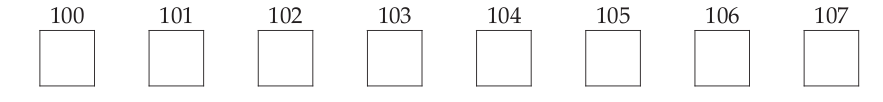
\includegraphics[scale=.3]{g1.png}
	\end{figure}
\begin{enumerate}
\item Cada localizaci\'on es llamado un \texttt{byte}.
\item  Cada localizaci\'on en memoria es identificado por una \'unica direcci\'on.
\item  Cada localizaci\'on en memoria contiene un valor.
\end{enumerate}

El siguiente gr\'afico muestra 5 valores enteros, cada uno ocupando una
cantidad de \texttt{bytes}. 

\begin{figure}[htbp]
	\centering
	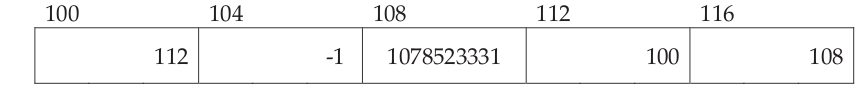
\includegraphics[scale=.3]{g2.png}
\end{figure}
\end{frame}

\begin{frame}[fragile]{}
	\Fontvi
$\bullet$ Los lenguajes de programaci\'on de alto nivel proporcionan la habilidad de
referirse a la localizaci\'on de memoria por nombres que por direcciones y esos nombres son llamados \texttt{variables}.

\begin{figure}[h]
	\centering
	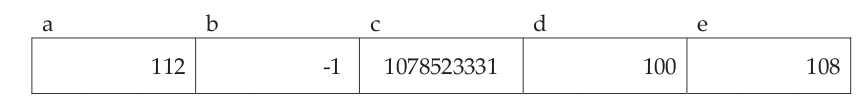
\includegraphics[scale=.3]{g3.png}
\end{figure}

Veamos las declaraciones de este gr\'afico

\begin{minted}{python}
int a= 112, b = -1;
float c = 3.14;
int *d = &a;
float *e = &c;
\end{minted}

Las variables \texttt{d} y \texttt{e} fueron declaradas como punteros y son inicialiazadas con la direcci\'on de otra variable. La inicializaci\'on es hecha con el operador \texttt{\&}, que produce la direcci\'on de memoria de su operando. 
\end{frame}

\begin{frame}[fragile]{}
	\frametitle{\textcolor{orange}{\hspace{4.0 cm} Punteros en C}}
	\Fontvi
\begin{enumerate}
\item Una variable puntero almacena la direcci\'on de una localizaci\'on de memoria que almacena el tipo al cual apunta.
 
 
\begin{minted}{python}
int *ptr   // almacena la direccion de un entero.
           // ptr 'apunta a' un int.
			           
char *cptr // almacena la direccion de un char.
           // cptr 'apunta a' un char.
\end{minted}
\item El tipo de \texttt{cptr} es un puntero a char. Este apunta a una localizaci\'on de memoria que almacena un valor char. Mediante \texttt{cptr} podemos acceder indirectamente un valor char. 
\begin{figure}[h]
	\centering
	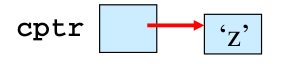
\includegraphics[scale=.42]{j1.png}
\end{figure}
\item El tipo de \texttt{ptr} es un puntero a un entero. Este apunta a una localizaci\'on de memoria que almacena un valor int.

\begin{figure}[h]
	\centering
	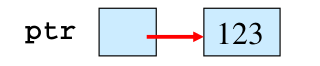
\includegraphics[scale=.42]{j2.png}
\end{figure}
\end{enumerate}
\end{frame}
\begin{frame}[fragile]{}
\frametitle{\textcolor{brown}{\hspace{2.0 cm} Inicializando variables puntero}}
\Fontvi

$\bullet$ Como una variable, se debe inicializar el puntero antes de que se pueda utilizar.

\vspace{0.2cm}

$\bullet$ Asigna la variable puntero el valor de una direcci\'on de memoria que pueda almacenar el tipo al cual apunta.


\begin{enumerate}
\item \textcolor{red}{NULL} es un especial valor para punteros. No es una direcci\'on v\'alida.

\begin{columns}
	\begin{column}{0.2\textwidth}
		\begin{minted}{c}
	 char *cptr = NULL;
		\end{minted}
	\end{column}
	\begin{column}{0.2\textwidth}
		\begin{figure}[h]
			\centering
			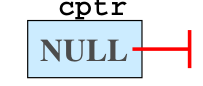
\includegraphics[scale=.3]{j3.png}
		\end{figure}
	\end{column}
	​  \end{columns}

\item El operador \texttt{\&} evalua la direcci\'on de una variable argumento.
\Fontvia
\begin{columns}
	\begin{column}{0.4\textwidth}
		\begin{minted}{c}
		int x = 3;
		int *ptr = NULL, *ptr2 = NULL;
		ptr = &x; // Consigue la direccion de x
		          // ptr 'apunta a' x 
		ptr2 = ptr; //ptr2 obtiene el valor de ptr
		  // ambos apunta a la misma localizacion
		char *cptr = &x; // ERROR!?. 
		\end{minted}
	\end{column}
	\begin{column}{0.2\textwidth}
		\begin{figure}[h]
			\centering
			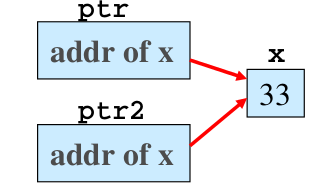
\includegraphics[scale=.3]{j4.png}
		\end{figure}
	\end{column}
	​  \end{columns}
\end{enumerate}
\end{frame}
\begin{frame}[fragile]{}
	\frametitle{\textcolor{blue}{\hspace{4.0 cm} El uso de punteros}}
\Fontvi
Una vez que un puntero es  inicializado  apuntando  a una localizaci\'on de almacenamiento v\'alido, se puede acceder al valor al que apunta usando el operador \textcolor{red}{*}
\Fontvia


\begin{Verbatim}
         * : dereferenciando una variable puntero
         (accede a la localizacion de almacenamiento a la que apunta.)
\end{Verbatim}

\begin{minted}{python}
ptr = &x; // ptr tiene la direccion de x 'ptr apunta a x'
*ptr = 10  // almacena 10 en la localizacion que ptr apunta
\end{minted}

\begin{figure}[h]
	\centering
	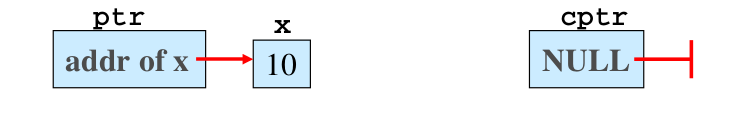
\includegraphics[scale=.3]{j5.png}
\end{figure}

\begin{minted}{python}
cptr = NULL;  
*cptr = `b`;   // cptr no apunta a una localizacion de almacenamiento 
               // char valida, tratando de dereferenciar cptr  
               // (un puntero NULL) se colgara el programa

if(cptr != NULL){ // Una mejor manera es probar para  NULL primero.
	*cptr = `b`;  // El ajuste del puntero NULL, permite probar 
	              // por un direccion invalida antes de la  desreferenciacion.
	}
\end{minted}
\end{frame}
\end{document}
